\chapter{文書のコンパイル}

\section{コンパイル}

文書をコンパイルする最も簡単な方法は、
「コンパイル」コマンドまたは「ビルド&表示」コマンド
(「コンパイル」ボタン - ショートカット:F6、
「ビルド&表示」ボタン - ショートカット:F1)を使用することである。
「TeXstudioの設定」ダイアログを通して既定のコマンドを選択することができる。

(また、「ツール」メニューで各々のコマンドを一つ一つ起動することも可能である。)

注:「ツールメニュー」の「補助ファイルの削除」で
LaTeXのコンパイル時に生成されるファイル(dvi, toc, aux\ldots{})を
削除することができる(ps&pdfファイルを除く)。


\begin{figure}[H]
  \centering
  
\includegraphics{compile_toolbar.png}
  \caption{コンパイルツールバー}
\end{figure}

\textbf{注意:すべてのファイルには拡張子がなければならず、
「タイトルなし」ファイルや名前に空白のあるファイルはコンパイルできない。}

\section{ログファイル}

「ビルド」コマンドで、
ログファイルが「メッセージ/ログファイル」パネルに自動的に表示される。
もしコンパイル時にエラーが生じれば「エラー」パネルにそのエラーが表示される。
「エラー」パネル上の「行」列の数字をクリックすれば、
エディタ上で対応する行にカーソルが移動して
そのエラーが「ログファイル」パネル上でも表示される。

\begin{figure}[H]
  \centering
  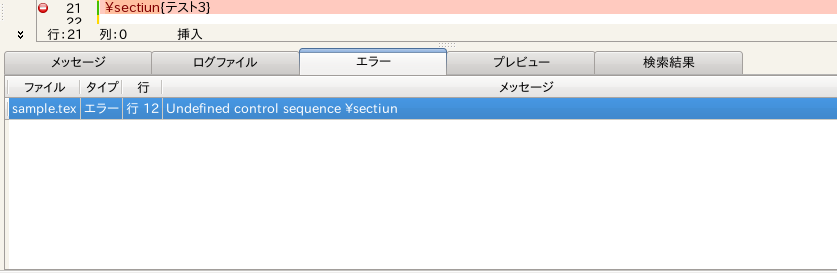
\includegraphics[width=.8\linewidth]{doc15.png}
  \caption{ログファイル}
\end{figure}

「次のエラー」と「前のエラー」コマンドでコンパイル中に検出されたエラーの間を移動できる。

エラーや警告、良くないボックスのある行は背景がそれぞれ赤、黄色、青で強調表示される。
また、Ctrl+Up/Downでそれらの間を移動できる
(エラーのみに対してはCtrl+Shift、警告のみに対してはCtrl+Alt、
良くないボックスのみに対してはAlt+Shiftを用いる)。

更に、それらの行へ移動するとツールチップで
間違いのさらなる詳細が表示される(行番号の左側の印にマウスを合わせた場合にも
表示される)。
